

In der Einleitung sollen zunächst ein paar Grundlegende Voraussetzungen dieser Projektgruppe geklärt werden. So wird in diesem Kapitel zunächst der Hintergrund sowie die Motivation der gesamten Projektgruppe erläutert, danach erfolgt noch eine kurze Projektbeschreibung. Abschließend sollen noch einige Formalien geklärt werden. Dies erfolgt mittels einer Gliederung des kompletten Projekthandbuches, und zuletzt mit einer Auflistung des beigefügten Anhanges.

% Unterkapitel
\subsection{Hintergrund und Motivation} \label{hintergrund-subsec}



Die Gesellschaft befindet sich seit mehreren Jahren in einem beschleunigten Wandel der das Leben ver{\"a}ndert. 
Dieser Wandel wurde durch die Automation und die Digitalisierung, welche sich beide erg{\"a}nzen verst{\"a}rkt und wird auch als vierte industrielle Revolution bezeichnet, die zu Ver{\"a}nderungen im Alltag als auch in der Wirtschaft gef{\"u}hrt hat. 
Durch die Digitalisierung mussten viele Branchen wie die Musik, Einzelhandel und die Logistik \& Versand Industrie umstrukturieren oder wurden wie zum Beispiel die Schreibmaschinenindustrie vollst{\"a}ndig beseitigt. 
Somit erscheinen t{\"a}glich technologische Innovationen, die im Internet, Fernsehen oder in Zeitschriften ver{\"o}ffentlicht werden. 
Ein Bereich sind die affektiven Technologien. 
Dieser Bereich hat sich als interdisziplin{\"a}res Forschungsfeld etabliert und untersucht die Interaktion zwischen Mensch und Maschine, wobei Emotionen im Mittelpunkt stehen und l{\"a}sst sich in zwei Systeme unterteilen. 
Zu einem die emotionssensitiven Technologien, womit Maschinen verstehen was Menschen f{\"u}hlen und zum anderen die ``Emotional Robotic''- Technologien, die einen Roboter menschen{\"a}hnlicher erscheinen lassen. 
Um die Forschung im Bereich emotionssensitiven Technologien voranzutreiben wurde ein Forschungsprojekt mit den Namen ``ELISE: Entwicklung von interaktiven und emotionssensitiven Lernsystemen zur Kompetenzerhaltung im Gesch{\"a}ftsprozessmanagement''  ins Leben gerufen (siehe Kapitel \ref{elise-subsec}).
Der Lehrstuhl Medizinische Informatik und Mikrosystementwurf entwickelt im Rahmen des Gesamtprojektes ein Sensorsystem, welches die Vital-, Elektroenzephalografie- und Elektrookulografiewerte aufzeichnet. 
Diese werden dann vom Lehrstuhl f{\"u}r Mustererkennung ausgewertet. 
Die Lerninhalte der Hauptanwendung des ELISE-Projekts werden daraufhin an Emotionen und Gem{\"u}tslagen der Lernenden wie Gl{\"u}ck, Langeweile, Frustration auf Basis von biomedizinischer Daten angepasst, um so den individuellen Erfolg des Lernenden zu erh{\"o}hen. 
Diese Projektarbeit befasst sich mit dem Entwurf eines kompakten mikrocontrollergest{\"u}tzten Systems zur Emotionserkennung in einer Virtual-Reality-Umgebung, Die Projektarbeit baut auf eine vorher am Lehrstuhl geschriebene Master Thesis  auf\cite{msckroenert} und ist eine Zusammenarbeit mit dem Lehrstuhl f{\"u}r Mustererkennung. 
Sie beinhaltet den Aufbau und die Programmierung des Mikrocontrollers, welches zur Kommunikation der verschiedenen biomedizinischen Sensoren dient, die Entwicklung der VR-Umgebung, die Schnittstellen zwischen Hardware und Software und die Speicherung der Rohdaten (Vital-, Elektroenzephalografie- und Elektrookulografiewerte). 
Diese Rohdaten wurden anhand von Messreihen an 88 Probanden gewonnen und wurden dem Lehrstuhl f{\"u}r Mustererkennung zur Verarbeitung {\"u}bergeben. 
Die Ergebnisse der Verarbeitung werden auch aufgef{\"u}hrt. 



% Unterkapitel
\subsection{ELISE Projektbeschreibung} \label{elise-subsec}


ELISE ist ein Verbundprojekt, welches die Entwicklung eines interaktives und emotionssensitiven Lernsystems zur Kompetenzentwicklung im Bereich der Gesch{\"a}ftsprozessmanagement plant. 
Hierf{\"u}r kamen f{\"u}nf Partner des Forschungskollegs (FoKoS) der Universit{\"a}t Siegen zusammen – der Lehrstuhl f{\"u}r Wirtschaftsinformatik \& Center for Responsible Innovation \& Design, die Forschungsgruppe Research Group for Pattern Recognition, der Lehrstuhl Medizinische Informatik und Mikrosystementwurf der Universit{\"a}t Siegen, der Spieleentwickler Limbic Entertainment GmbH und der Softwarehersteller Software AG. 
Zusammen befassen sie sich mit einem interaktiven und emotionssensitiven Lernsystems in Form eines Spiels, das in einer virtuellen Umgebung erfolgt. 
Zudem befasst sich das Projekt mit der Auswirkung von solcher Systeme hinsichtlich ethischer und gesellschaftlicher Aspekte auf die Akzeptanz potenzieller Nutzerinnen und Nutzer.
Abbildung \ref{fig-elise} zeigt das vorhaben, welches durch das Projekt Elise verwirklicht werden soll.


\begin{figure}[H] \centering
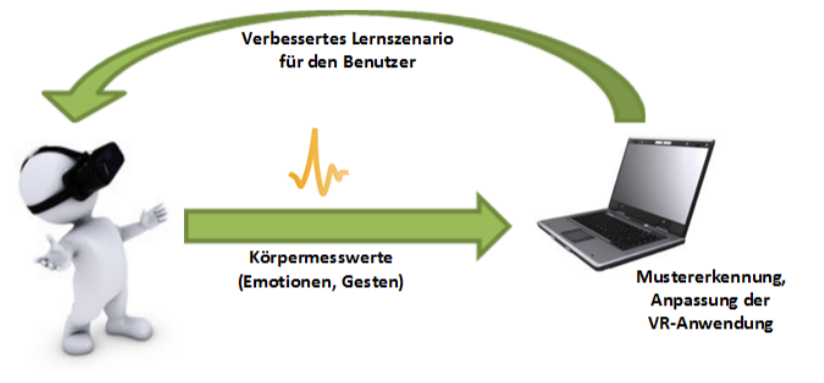
\includegraphics[width=12cm]{Images/elise_projektbeschreibung.png} 
\vspace{-0.3cm} 
\caption{Grobe {\"U}bersicht des Gesamtprojekts\cite{msckroenert}.}
\label{fig-elise} 
\end{figure}

Der Lehrstuhl Medizinische Informatik und Mikrosystementwurf entwickelt im Rahmen des Gesamtprojektes ein Sensorsystem, welches die Vital-, Elektroenzephalografie-, Elektrookulografie- und galavanische Hautreaktionwerte aufzeichnet. 
Diese werden dann vom Lehrstuhl f{\"u}r Mustererkennung ausgewertet. 
Die Lerninhalte der Hauptanwendung des ELISE-Projekts werden daraufhin an Emotionen und Gem{\"u}tslagen der Lernenden wie Gl{\"u}ck, Langeweile, Frustration auf Basis von biomedizinischer Daten angepasst, um so den individuellen Erfolg des Lernenden zu erh{\"o}hen.

% Unterkapitel
\subsection{Gliederung dieser Dokumentation} \label{gliederung-subsec}


Die Dokumentation ist in mehreren Teil gegliedert: eine Einführung, die Entwicklung des ersten Prototypen, die Entwicklung des zweiten Prototypen, die Entwicklung des dritten/finalen Prototypen und ein Schlussteil. \\

Einführung: \\

Die Dokumentation fängt mit einer Einleitung an, die den Hintergrund und die Motivation, die Elise Projektbeschreibung, die Gliederung dieser Dokumentation und den mit der Dokumentation übergebenen Anhang erläutert (geschrieben von Minas Michail). 
Der nächste Punkt ``Organisation'' beinhaltet zum einen die Verantwortungsbereiche der aufgeteilten Aufgaben innerhalb der Gruppe und  zum anderen wird erläutert wie und wann die Gruppentreffen stattgefunden haben (geschrieben von Artur Piet). 
Daraufhin werden die Grundlagen übermittelt, um späteres geschehen in der Dokumentation besser nach voll ziehen zu können. 
Der Punkt Grundlagen enthält die Definition von Emotionen (geschrieben von Arnaud Eric Toham Waffo), die Grundlagen der verwendeten Hardware und Software (geschrieben von Arnaud Eric Toham Waffo), die Grundlagen der verwendeten Sensoren und biophysiologischen Signale (geschrieben von Kevin Orth), die Grundlagen der Kommunikation zwischen den gewonnen Sensordaten und dem Board (geschrieben von Kevin Orth \& Jonas Pöhler), die Grundlagen der Mustererkennung (geschrieben von Artur Piet) und die Grundlagen zur Emotionserkennung (geschrieben von Artur Piet). 
Nach den Vermittlungen der Grundlagen \\

Entwicklung des ersten Prototypen: \\

Die Entwicklung des ersten Prototypen umfasst den Systementwurf und das Konzept der Hardware (geschrieben von Kevin Orth), die entwickelte Software zurKommunikation (geschrieben von Kevin Orth \& Jonas Pöhler), die Emotionsinduktion (geschrieben von Meryem Dural, Boris Kamdem \& Minas Michail), die Messreihe (geschrieben von Kevin Orth \& Artur Piet), die Musterkennung (geschrieben von Artur Piet) und die gewonnen Ergebnisse (geschrieben von Artur Piet). \\

Entwicklung des zweiten Prototypen: \\

Die Entwicklung des zweiten Prototypen umfasst den Systementwurf und das Konzept der Hardware und die modifizierte Software zur Kommunikation (beides  geschrieben von Kevin Orth \& Jonas Pöhler). 
Parallel zur Fertigstellung des zweiten Prototypen, lief die Entwicklung der Emotionsinduktion für den dritten Prototypen. \\

Entwicklung des dritten Prototypen: \\

Die Entwicklung des dritten Prototypen umfasst den Systementwurf und das Konzept der Hardware (geschrieben von Kevin Orth), die entwickelte Software zurKommunikation (geschrieben von Kevin Orth \& Jonas Pöhler), die Emotionsinduktion (geschrieben von Meryem Dural, Boris Kamdem \& Minas Michail), die Messreihe (geschrieben von Kevin Orth \& Artur Piet), die Musterkennung (geschrieben von Artur Piet) und die gewonnen Ergebnisse (geschrieben von Artur Piet). \\

Schlussteil: \\

Der Schlussteil beinhaltet das Kapitel Alternative Lösungen aufgeteilt in Kalibrierung (geschrieben von Jonas Pöhler) und Plan B (geschrieben von Meryem Dural) und eine Zusammenfassung (geschrieben von Arnaud Eric Toham Waffo) sowie einen Ausblick (geschrieben von Boris Kamdem).

% Unterkapitel
\subsection{Anhang}  \label{anhang-subsec}


Der Anhang enthält alle Dateien, die im Rahmen dieser Projektgruppe erstellt wurden, und wird in Form einer beigelegten CD-Rom zur Verfügung gestellt.
Bei diesen Dateien handelt es sich im Wesentlichen um die erstellten Eagle-Dateien (Schaltplan und Layout) die Dateien für den 3 Druck (Maske und Gehäuse) sowie den erstellten Code für den Mikrocontroller und die zu verarbeitende Software.
Zuletzt sind noch alle erstellten Anleitungen, für den Hardwareaufbau und die Versuchsdurchführung enthalten. Eine genaue Beschreibung der in den erwähnten Dateien behandelten Themen erfolgt in den nachfolgenden Kapiteln.
Auf der CD-Rom befinden sich im Ordner Senfemo-Anhang die folgenden Dateien:
\newline
-Eagle-Dateien aller drei Prototypen
\\
-Code für die Prototypen
\\
-Datenblätter der verwendeten Komponenten
\\
-Dateien für den 3D-Druck
\\
-diverse Anleitungen 
